\documentclass{report}
\usepackage{polski}
\usepackage[utf8]{inputenc}
\usepackage{graphicx}
\usepackage{url}
\usepackage{enumerate}
\title{Giełda}
\author{Szymon Stefański}
\begin{document}
\maketitle
\tableofcontents
\newpage
\chapter{Wstęp}
\section{Podstawowe pojęcia}
\subsection{Czym jest giełda?}
\textbf{Giełda}\cite{gielda} – organizowane w ustalonym miejscu i czasie spotkania handlowe, na których sprzedawane są ściśle określone towary po cenach ogłoszonych w codziennych notowaniach. Transakcje\footnote{ czynność zachodząca między sprzedającym i kupującym, która ma na celu wymianę towaru lub usługi. Transakcja finansowa kończy się umową sprzedaży. } na giełdach zawierane są zgodnie z obowiązującym regulaminem, między członkami giełdy pośredniczącymi w zawieraniu transakcji.
\subsection{Organizacja giełdy}
Giełda jest kontrolowana przez państwo, które udziela koncesji na jej działanie i określa sposób jej działania.
Giełdy można podzielić na dwie kategorie:
\begin{itemize}
\item giełda państwowa
\item giełda korporacyjna.
\end{itemize}
W pierwszym przypadku państwo jest jedynym właścicielem giełdy i decyduje o wszystkim co jest związane z jej działaniem. W drugim przypadku giełdę tworzymy w oparciu o normy prawa handlowego.Rynek papierów wartościowych, który jest tworzony przez banki, domy maklerskie, fundusze inwestycyjne i inne instytucje jest instytucją, na którą państwo nie ma bezpośredniego wpływu.
\newline Do prawidłowego funkcjonowania giełdy muszą zostać spełnione pewne warunki:
\begin{itemize}
\item określanie uczestników giełdy,
\item stworzenie statutu i regulaminu,
\item ustalić strukturę organizacyjną,
\item dysponować odpowiednim wyposażeniem materialnym.
\end{itemize}
\section {Rodzaje giełd}
Giełdy możemy dzielić według zasięgu geograficznego:
\begin{itemize}
\item regionalne;
\item krajowe;
\item międzynarodowe;
\end{itemize}
Oraz według zakresu rzeczowego transakcji:
\begin{itemize}
\item giełda towarów,
\item giełda instrumentów finansowych ,
\item giełda usług.
\end{itemize}
{\Large \textit{Giełda towarów}}
\newline Giełda towarów to rynek, na którym zawierane są transakcje towarów masowych, które mają wspólne cechy. Dokonuje się transakcji bez fizycznej obecności towarów, a jedynie na podstawie ich charakterystyki opisanej w kontrakcie. Deponujący jako potwierdzenie otrzymuje kwit składowy, który może być przedmiotem obrotu na giełdzie.
\newline {\Large \textit{Giełda instrumentów finansowych}}
\newline Giełda instrumentów finansowych polega na kupnie lub sprzedaży akcji. Obroty tej giełdy są większe od obrotów na giełdzie towarów czy usług. Głównymi podmiotami uczestniczącymi są banki, władze monetarne państwa, przedsiębiorstwa oraz osoby fizyczne.
\newline {\Large \textit{Giełda usług}}
\newline Przedmiotem kontraktu na międzynarodowych giełdach usług są przede wszystkim usługi transportowe, ubezpieczeniowe i pośrednictwo transakcyjne.
\newpage
\chapter{Inwestowanie na giełdzie}
\section{Czynniki sukcesu na giełdzie}
Według badań przeprowadzonych przez strefainwestorow.pl\cite{badania13} okazuje się, że do osiągnięcia sukcesu znaczenia nie ma posiadanie odpowiedniej strategii czy wiedza na temat analizowania rynku i spółek, a czynniki psychologiczne takie jak umiejętność opanowania emocji oraz bycie zdyscyplinowanym i konsekwentnym. Posiadanie tych cech nie zagwarantuje jednak pewnego sukcesu jeśli nie będzie się poświęcać wystarczającego czasu oraz nie będzie się miało odpowiedniej strategii inwestycyjnej. Każdy z tych czynników w mniejszym lub większym stopniu wpływa na sukces, który chce się osiągnąć. Nie ma więc jednego prawidłowego sposobu na wzrost kapitału.
\begin{figure}[h]
\centering
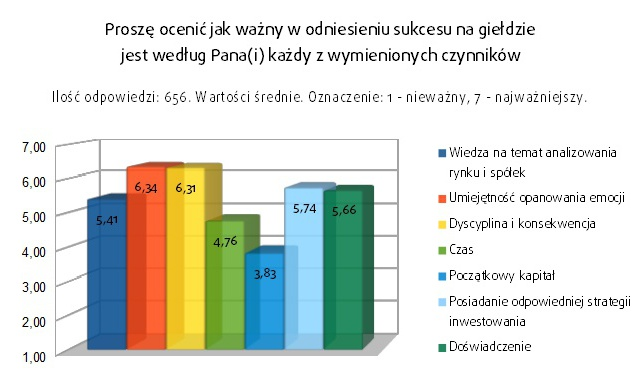
\includegraphics[scale=0.48]{obraz1}
\caption{Średnie oceny czynników sukcesu na giełdzie według ankietowanych. Źródło: badanie przeprowadzone przez StrefaInwestorow.pl}
\end{figure}
\newline Posiadanie tych cech nie zagwarantuje jednak pewnego sukcesu jeśli nie będzie się poświęcać wystarczającego czasu oraz nie będzie się miało odpowiedniej strategii inwestycyjnej. Każdy z tych czynników w mniejszym lub większym stopniu wpływa na sukces, który chce się osiągnąć. Nie ma więc jednego prawidłowego sposobu na wzrost kapitału.
\section{Pierwsze inwestycje}
Przy rozpoczęciu przygody z giełdą bardzo ważny jest wybór firm, w które chemy inwestować. Należy wybrać ich kilka aby nie stracić wszystkiego w razie potknięcia.Warto jest inwestować w dziedzinę, na której się znamy aby jak najłatwiej przewidzieć przyszłe zmiany na giełdzie. Pierwszą rzeczą, którą chcemy zrobić to zlecić kupno akcji w pewnej cenie. Jeżeli znajdzie się osoba, która po drugiej stronie w takiej cenie zechce je sprzedać dochodzi do transakcji, w której broker pobiera prowizję.
Od tej pory śledzimy notowania naszych akcji, ponieważ każda zmiana oznacza stratę lub zysk. Sprzedać akcje możemy w dowolnym momencie. Najczęściej dzieje się to przy dużym zysku akcji lub podczas spadania wartości aby ograniczyć straty. Rozpoczęcie przygody z giełdą nie jest trudne. Internetowy dostęp do rachunku inwestycyjnego pozwala  zarządzać funduszami w domowym zaciszu. Koszty bycia inwestorem giełdowym ograniczają się zazwyczaj do prowizji od wartości transakcji oraz podatku od zysku.
\begin{figure}[h]
\centering
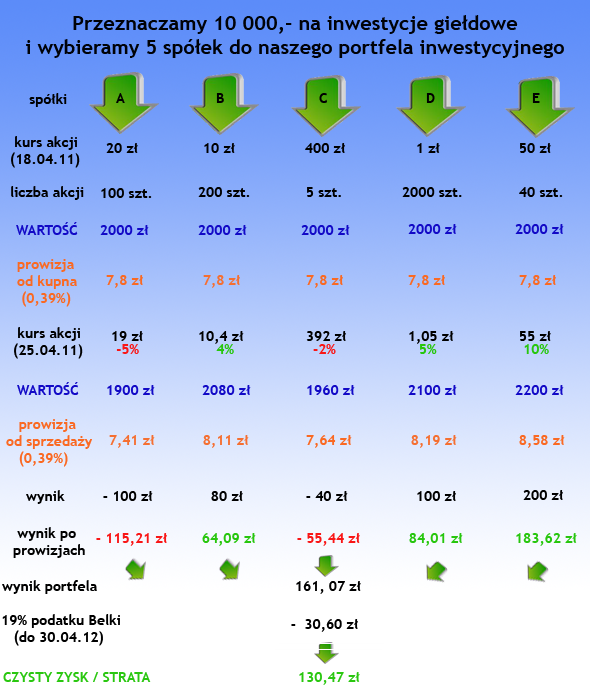
\includegraphics[scale=0.6]{tabela}
\caption{Symulacja inwestycji 10 000 zł w 5 spółek giełdowych.\cite{sym11}}
\end{figure}
\newpage
\chapter{Strategie Inwestycyjne}
\section{Kupno akcji w IPO}
Initial Public Offering\cite{perz2008sztuka} (IPO) polega na kupowaniu ofert publicznych, które pojawiają się na rynku po raz pierwszy i sprzedaży na pierwszej sesji, podczas których są notowane na giełdzie. Ta metoda zapewnia ponadprzeciętną stopę zwrotu.
\newline
\begin{table}[h]
\begin{tabular}{|c|c|c|} \hline
Wielkość badanej próby & Badany okres & Średnia stopa zwrotu w \% \\
\hline
13308 & 1960-1996 & 15,5 \\
\hline
2133 & 1959-1990 & 10,9 \\
\hline
170 & 1978-1992 & 10,9 \\
\hline
226 & 1989-1996 & 388,0 \\
\hline
79 & 1987-1991 & 48,5 \\
\hline
347 & 1980-1990 & 78,1 \\
\hline
\end{tabular}
\caption{Tabela przedstawiająca zysk używając metody IPO}
\end{table}
\section{Transakcje arbitrażowe}
Arbitraż\cite{perz2008sztuka} jest strategią pozwalającą na zarabianie bez ryzyka. Sytuacje klasycznego arbitrażu zdarzają się na rynku stosunkowo rzadko. Możliwość takich transakcji związane są z zaniżoną ceną niektórych instrumentów finansowych. Najczęściej wykorzystuje się przy tej strategii programy, które wychwytują większość okazji i automatycznie dokonują transakcji.
\newpage
\listoffigures
\listoftables
\bibliographystyle{plain}
\bibliography{bib}
\end{document}